

\documentclass[table]{beamer}
\usepackage{xcolor}
\usepackage[T1]{fontenc}
\usepackage[polish]{babel}
\usepackage[utf8]{inputenc}
\usetheme{Antibes}

\usepackage{array}

\usepackage{multirow}
\usepackage{listings}
\usepackage{longtable}


\title{PAKIET ARRAY}
\subtitle{tworzenie tabel w LaTeX'ie}
\author{Adam Czerwiński i Jakub Karmański}
\institute{POLSL}
\date{28.10.2019}
 
\renewcommand*\contentsname{Summary}

\begin{document}
 
\maketitle
 
\tableofcontents

\section{Wprowadzenie}
\begin{frame}[fragile]
Array to pakiet do LaTeX’a który udostępnia narzędzia do produkowania rozbudowanych tabel. 
Same tabele nie potrzebują pakietu 'array' do stworzenia tablicy, lecz w przypadku chęci ingerowania w np. długość czy kolor komórek pakiet ten jest wymagany.

W celu jego dodania do naszego pliku używamy:

\begin{lstlisting}
\usepackage{array}
\end{lstlisting}
\end{frame}

\begin{frame}[fragile]

Aby zdefiniować tablice:
\begin{lstlisting}
\begin{tabular}
\end{tabular} 
\end{lstlisting}
To oświadcza, że w tabeli zostaną użyte trzy kolumny oddzielone pionową linią. Każde c oznacza, że zawartość kolumny zostanie wyśrodkowana, możesz także użyć r, aby wyrównać tekst do prawej i l, aby wyrównać do lewej:
\begin{lstlisting}
{ |c|c|c| }
\end{lstlisting}
Spowoduje to wstawienie poziomej linii na górze stołu i na dole. Nie ma ograniczeń co do liczby przypadków użycia \ hline :
\begin{lstlisting}
\hline
\end{lstlisting}
Każdy 'Et' jest separatorem komórek, a podwójny ukośnik \\ ustawia koniec tego wiersza.
\begin{lstlisting}
cell1 & cell2 & cell3 \\
\end{lstlisting}
\end{frame}

\section{Tworzenie prostej tabeli w LaTeX}
\begin{frame}[fragile]
 
Poniżej możemy zobaczyć najprostszy działający przykład tabeli bez użycia pakietu array

\begin{lstlisting}
\begin{tabular}{ c c c }
 cell1 & cell2 & cell3 \\ 
 cell4 & cell5 & cell6 \\  
 cell7 & cell8 & cell9    
\end{tabular}
\end{lstlisting}

\begin{center}
\begin{tabular}{ c c c }
 cell1 & cell2 & cell3 \\ 
 cell4 & cell5 & cell6 \\  
 cell7 & cell8 & cell9    
\end{tabular}
\end{center} 

Gdzie { c c c } - jest definicją kolumn naszej tablicy.Litera 'c' pochodzi od słowa 'center' i jest ona wymagana podczas definiowania kolumn naszej tablicy
 
\end{frame}

\begin{frame}[fragile]

Obramowanie:
\begin{lstlisting}
\begin{tabular}{ |c|c|c| } 
 \hline
 cell1 & cell2 & cell3 \\ 
 cell4 & cell5 & cell6 \\ 
 cell7 & cell8 & cell9 \\ 
\end{tabular}
\end{center}
\end{lstlisting}

\begin{center}
\begin{tabular}{ |c|c|c| } 
 \hline
 cell1 & cell2 & cell3 \\ 
 cell4 & cell5 & cell6 \\ 
 cell7 & cell8 & cell9 \\ 
\end{tabular}
\end{center}
\end{frame}

\section{Tablice o stałej długości}

\begin{frame}[fragile]
\begin{lstlisting}
\begin{tabular}{ | m{1cm} | m{1cm}| m{1cm} | } 
\hline
cell1 dummy text dummy text dummy text& cell2 & cell3 \\ 
\hline
cell1 dummy text dummy text dummy text & cell5 & cell6 \\ 
\hline
cell7 & cell8 & cell9 \\ 
\hline
\end{tabular}
\end{lstlisting}
\end{frame}

\begin{frame}
 \begin{center}
\begin{tabular}{ | m{2cm} | m{1cm}| m{3cm} | } 
\hline
cell1 & cell2 & cell3 \\ 
\hline
cell1 & cell5 & cell6 \\ 
\hline
cell7 & cell8 & cell9 \\ 
\hline
\end{tabular}
\end{center}
\end{frame}

\section{Lączenie kolumn i wierszy}



\begin{frame}
\begin{center}
\begin{tabular}{ |p{2cm}|p{2cm}|p{2cm}|  }
 \hline
 \multicolumn{3}{|c|}{Połączenie 3 kolumn} \\
 \hline
 Kol1&Kol2&Kol3\\
 \hline
 1 & 2 & 3\\
 1 & 2 & 3\\
 1 & 2 & 3\\
 1 & 2 & 3\\
 \hline
\end{tabular}
\end{center}
\end{frame}

\begin{frame}

 multicolumn  {3}  {|c|}  {Połączenie 3 kolumn}
 
 usepackage	{multirow}
\end{frame}

\section{Tabele wielostronicowe}
\begin{frame}[fragile]
 
Zachowanie longtable jest podobne do domyślnego tabelarycznego, ale generuje tabele, które można podzielić za pomocą standardowego algorytmu podziału strony LATEX. Istnieją cztery elementy specyficzne dla longtable.
\end{frame}

\begin{frame}

1.endfirsthead\\
Wszystko powyżej tego polecenia pojawi się na początku tabeli, na pierwszej stronie.\\

2.endhead\\
Cokolwiek umieścisz przed tym poleceniem i poniżej endfirsthead, wyświetli się u góry tabeli na każdej stronie oprócz pierwszej.\\

3.endfoot\\
Podobnie jak endhead, to co umieścisz po endhead i przed tym poleceniem pojawi się na dole tabeli na każdej stronie oprócz ostatniej.\\

4.endlastfoot\\
Podobne do endfisthead. Elementy po endfoot i przed tym poleceniem będą wyświetlane na dole tabeli, ale tylko na ostatniej stronie, na której pojawia się tabela.\\
Przykład w pliku...
\end{frame}

\section{Pozycjonowanie tablic}
\begin{frame}[fragile]
Aby pozycjonować tabelę, musi ona zostać umieszczona w środowisku table. Poniższa tabela jest pozycjonowana ``tutaj``, za pomocą opcjonalnego parametru ''h!''.
{\small
\begin{lstlisting}

\begin{table}[h!]
\centering
	\begin{tabular}{| c | c | c | c |} 
 		\hline
 		Col1 & Col2 & Col2 & Col3 \\ 
 		\hline \hline
 		1 & 6 & 837 & 787 \\ 
		2 & 7 & 78 & 515 \\
 		3 & 545 & 778 & 707 \\
 		4 & 545 & 144 & 760 \\
 		5 & 88 & 788 & 64 \\ 
 		\hline
 	\end{tabular}
\end{table}

\end{lstlisting}
}
\end{frame}

\begin{frame}

Innymi parametrami pozycjonowania są jeszcze:
\begin{itemize}
	\item \textbf{h} - umieści tabelę ''tutaj'' - gdzie kod źródłowy
	\item \textbf{t} - umieści tabelę na górze strony
	\item \textbf{b} - umieści tabelę na dole strony
	\item \textbf{p} - umieści tabelę na specjalniej stronie, tylko dla tabel
	\item \textbf{!} - nadpisuje domyślny parametr \LaTeX do określenia pozycji za pomocą liczb zmiennoprzecinkowych
	\item \textbf{H} - umieszcza tabelę w wyznaczonej lokalizacji. Podobne do h!.
\end{itemize}

\end{frame}



\section{Podpisy, etykiety i odniesienia}
\begin{frame}
Tabele mogą zawierać podpis oraz etykietę do której można się odnieść.

Tabela \ref{table:tabela1} jest przykładem do odniesienia się do elementu \LaTeX.

\begin{table}[h!]
\centering
\begin{tabular}{||c c c c||} 
 \hline
 Col1 & Col2 & Col2 & Col3 \\ [0.5ex] 
 \hline\hline
 1 & 6 & 87837 & 787 \\ 
 2 & 7 & 78 & 5415 \\
 3 & 545 & 778 & 7507 \\
 4 & 545 & 18744 & 7560 \\
 5 & 88 & 788 & 6344 \\ [1ex] 
 \hline
\end{tabular}
\caption{Przykładowa tablica}
\label{table:tabela1}
\end{table}
\end{frame}

\begin{frame}[fragile]
Jeżeli chcemy oznaczyć tabelę, użyjemy do tego elementu label:
\begin{lstlisting}
\label{table:tabela1}
\end{lstlisting}
Aby się odnieść do oznaczonego elementu, użyjemy referencji:
\begin{lstlisting}
\ref{table:tabela1}
\end{lstlisting}
Aby podpisać tabelę, użyjemy elementu caption:
\begin{lstlisting}
\caption{Przykladowa tablica}
\end{lstlisting}
\end{frame}


\begin{frame}[fragile]
\small{
\begin{lstlisting}
Tabela \ref{table:tabela1} jest przykladem do
odniesienia sie do elementu \LaTeX.

\begin{table}[h!]
\centering
\begin{tabular}{||c c c c||} 
 \hline
 Col1 & Col2 & Col2 & Col3 \\ [0.5ex] 
 \hline\hline
 1 & 6 & 87837 & 787 \\ 
 2 & 7 & 78 & 5415 \\
 3 & 545 & 778 & 7507 \\
 4 & 545 & 18744 & 7560 \\
 5 & 88 & 788 & 6344 \\ [1ex] 
 \hline
\end{tabular}
\caption{Przykladowa tablica}
\label{table:tabela1}
\end{table}

\end{lstlisting}
}

\end{frame}




\section{Lista tabel}
\begin{frame}[fragile]
Aby wylistować wszystkie tabele zawarte w dokumencie, które zawierają element label, użyjemy do tego 
\begin{verbatim}
\listoftables
\end{verbatim}
Nazwa nagłówka zostanie dostosowana do do języka używanego przez pakiet \textbf{babel}\\
Przykład:
\begin{figure}
	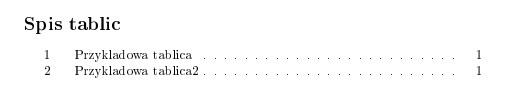
\includegraphics[scale=.6]{spis_tablic.png}
	\caption{Spis tablic w dokumencie}
\end{figure}
\end{frame}








\section{Zmiana wyglądu tabeli}
\begin{frame}[fragile]
Istnieje możliwość zmiany wygląd niektórych elementów tabeli, między innymi:
\begin{itemize}
	\item grubość linii
	\item kolor linii
	\item kolor tła komórek w tabeli
	\item odstęp tekstu od ścian komórki (padding)
	\item wysokość komórek
	\item i inne.. 
\end{itemize}


\end{frame}

\begin{frame}[fragile]
Aby ustawić grubość obramowania 1mm, użyjemy do tego:
\begin{verbatim}
\setlength{\arrayrulewidth}{1mm}
\end{verbatim}


Aby ustawić odstęp pomiędzy lewą i prawą krawędzią, a tekstem:
\begin{verbatim}
\setlength{\tabcolsep}{18pt}
\end{verbatim}

Aby ustawić wysokość komórek równą 150\% domyślnej wartości: 
\begin{verbatim}
renewcommand{\arraystretch}{1.5}
\end{verbatim}


\end{frame}


\begin{frame}

\setlength{\arrayrulewidth}{1mm}
\setlength{\tabcolsep}{15pt}
\renewcommand{\arraystretch}{1.1}

\centering
Przykładowa tabela

\begin{center}


\begin{tabular}{ |p{2.2cm}|p{2.2cm}|p{2.2cm}|  }
\hline
\multicolumn{3}{|c|}{Country List} \\
\hline
Country Name     or Area Name& ISO ALPHA 2 Code &ISO ALPHA 3 \\
\hline
Afghanistan & AF &AFG \\
Aland Islands & AX   & ALA \\
Albania &AL & ALB \\
Algeria    &DZ & DZA \\
American Samoa & AS & ASM \\
Andorra & AD & AND   \\
Angola & AO & AGO \\
\hline
\end{tabular}
\end{center}

\end{frame}

\begin{frame}[fragile]
Aby zwiększyć czytelność tabeli, można zastosować naprzemienne kolorowanie wierszy. Aby tego dokonać, potrzebujemy użyć pakietu xcolor wraz z parametrem table.
\begin{verbatim}
\usepackage[table]{xcolor}
\end{verbatim}

\begin{center}
\setlength{\arrayrulewidth}{1mm}
\arrayrulecolor[HTML]{DB5800}
{\rowcolors{3}{green!20!red!50}{green!70!yellow!40}
	\begin{tabular}{| c | c | c | c |} 
 		\hline
 		t & t & Col2 & Col3 \\ 
 		\hline \hline
 		\rowcolor{lightgray} 1 & 6 & 837 & 787 \\ 
		2 & 7 & 78 & 515 \\
 		3 & 545 & 778 & 707 \\
 		4 & 545 & \cellcolor{blue} 144 & 760 \\
 		5 & 88 & 788 & 64 \\ 
 		\hline
 	
 	\end{tabular}
}
\end{center}

\end{frame}


\begin{frame}[fragile]

W powyższym przykładzie użyto następnego kodu:
\begin{verbatim}
{\rowcolors{3}{green!20!red!50}{green!70!yellow!40} ... }
\end{verbatim}
Gdzie kropki oznaczają definicję tabeli.\\
Pierwszy parametr ''3'' oznacza wiersz, od którego zacząć kolorowanie.\\
Drugi parametr oznacza kolor dla nieparzystych wierszy.\\
Trzeci parametr oznacza kolor dla parzystych wierszy.\\
Wartości w drugim i trzecim parametrze oznaczają proporcje kolorów.\\

\end{frame}

\begin{frame}[fragile]
Pierwszy wiersz różni się kolorem od podanych powyżej, ponieważ nadpisaliśmy jego kolor poprzez element ''rowcolor'' tuż przed podaniem tekstu w wierszu.
\begin{verbatim}
\rowcolor{lightgray} 1 & 6 & 837 & 787 \\ 
\end{verbatim}
Jedna z komórek jest niebieska, użyto do tego ''cellcolor''
\begin{verbatim}
4 & 545 & \cellcolor{blue} 144 & 760 \\
\end{verbatim}
Kolor obramowania zmieniliśmy za pomocą ''arrayrulecolor'' przed definiowaniem tabeli
\begin{verbatim}
\arrayrulecolor[HTML]{DB5800}
\end{verbatim}
Użyto tutaj formatu \textbf{HTML RRGGBB}, jednak można użyć innych formatów.
\end{frame}



\section{Linki}
\begin{frame}
 https://www.overleaf.com/learn/latex/Tables
\end{frame}

\section{Zadanie}

\begin{frame}
 \begin{enumerate}
 	\item Utworzyć tabelę(3 kolumny), w której tekst wewnątrz komórek będzie wyrównany do lewej,prawej oraz wyśrodkowany. 
 	\item Utworzyć tabelę z połączonymi kolumnami oraz wierszami (min jedno połączenie 2 kolumn i 2 wierszy)
 	\item Utworzyć tabelę z pozycjonowaniem na ''here'' i ''top'', która zawiera etykietę, podpis oraz odwołać się do niej oraz utworzyć listę tabel zawartych w dokumencie.
 	\item Utworzyć tabelę, która:
 		\begin{itemize}
 			\item ma grubość obramowania wynoszącą 0.7mm
 			\item ma padding równą 15pt
 			\item wysokość komórek wynosi 130\% domyślnej wartości
 		\end{itemize}
 	\item Pokolorować tabelę, której wiersze będą miały naprzemiennie inny kolor.
 	Wyróżnić komórki nadając im inny kolor oraz zmienić kolor obramowania.
 \end{enumerate}
\end{frame}

\end{document}